\documentclass{article}
\usepackage{tikz}
\usepackage{amsmath}
\usepackage{amsthm}
\usepackage{MnSymbol}
\usepackage{upgreek}
\usepackage{etoolbox}
\usepackage{mathtools}
\usepackage{makeidx}
\usepackage{hyperref}
\usepackage{amsfonts}
\title{Trabajo Pr\'actico 3: Map-Reduce}
\author{Mart\'{i}n Arjovsky 683/12 \\ Ezequiel Dar\'io Gambaccini 715/13 \\ Silvio Vileri\~no 106/12}
\date{Julio 2014}

\usepackage{listings}
\usepackage{color}
\definecolor{lightgray}{rgb}{.9,.9,.9}
\definecolor{darkgray}{rgb}{.4,.4,.4}
\definecolor{purple}{rgb}{0.65, 0.12, 0.82}

\lstdefinelanguage{JavaScript}{
  keywords={typeof, new, true, false, catch, function, return, null, catch, switch, var, if, in, while, do, else, case, break},
  keywordstyle=\color{blue}\bfseries,
  ndkeywords={class, export, boolean, throw, implements, import, this},
  ndkeywordstyle=\color{darkgray}\bfseries,
  identifierstyle=\color{black},
  sensitive=false,
  comment=[l]{//},
  morecomment=[s]{/*}{*/},
  commentstyle=\color{purple}\ttfamily,
  stringstyle=\color{red}\ttfamily,
  morestring=[b]',
  morestring=[b]"
}

\lstset{
   language=JavaScript,
   backgroundcolor=\color{lightgray},
   extendedchars=true,
   basicstyle=\footnotesize\ttfamily,
   showstringspaces=false,
   showspaces=false,
   numbers=left,
   numberstyle=\footnotesize,
   numbersep=9pt,
   tabsize=2,
   breaklines=true,
   showtabs=false,
   captionpos=b
}


\makeindex

\begin{document}
\maketitle

\section{Encontrar las mejores pel\'iculas}

 Se requer\'ia obtener la lista de las 12 pel\'iculas mejor rankeadas con m\'as de 20 reviews. Para esto, lo que decidimos hacer fue que en el map se emitiera el id del producto con un objeto que conten\'ia el puntaje de la review y una variable count inicializada a 1.
\\ En el siguiente paso, reduce, lo que se hace es sumar todos los objetos {puntaje, cantidad} y emitir el resultado.
\\ Finalmente, en el finalize, se filtra aquellas peliculas que tienen count $>$ 19. Para las pel\'iculas que tienen m\'as de 19 rese\~nas se devuelve la sumatoria de puntajes dividida la cantidad de rese\~nas.
\\ Para las que tienen menos de 20 rese\~nas se devuelve -1.
\\ Luego, usando un script de python para parsear la salida de runner.py, se filtra aquellas peliculas que su puntaje promedio es distinto de -1, y luego se las ordena en orden decreciente por puntaje, quedandose con las primeras 12.

Las pel\'iculas que obtuvimos con sus respectivos puntajes y nombres (conseguidos a trav\'es del buscador de Amazon) fueron:

\begin{itemize}
\item B00000JSJ5, 5.0, All Creatures Great and Small, Series 2: Volumes 1-6
\item B00004YKS6, 5.0, Genghis Blues
\item B00004YKS7, 5.0, Genghis Blues
\item B0002NY7UY, 5.0, Live in Concert (Dion)
\item B0007GAEXK, 5.0, The Mole - The Complete First Season
\item B0007Z4HAC, 5.0, Salsa Crazy Presents: Learn to Salsa Dance, Intermediate Series, Volume 1
\item B000AOEPU2, 5.0, WWE: Bret "Hitman" Hart - The Best There Is, The Best There Was, The Best There Ever Will Be
\item B000MCIADA, 5.0, A Reiki 1st, Aura and Chakra Attunement Performed
\item B003YBGJ4S, 5.0, WELL worked out with Tannis
\item B004LK24BI, 5.0, 50/50 Cardio and Weights with Angie Gorr
\item B006JN87UC, 5.0, Transformers: Prime - Season One
\item B008COIZHQ, 5.0, Genghis Blues
\item B005FY0FPG, 4.987012987012987, Dream With Me in Concert
\item B000M7XRC4, 4.977777777777778, The Venture Bros. - Season Two
\end{itemize}

A continuaci\'on se muestra el c\'odigo de map, reduce y finalize respectivamente.

\begin{lstlisting}
function () {
  data = {};
  data.score = parseFloat(this.score,10);
  data.count = 1;
  emit(this.productId, data);
}

function (key, values) {
  var res = {};
  res.score = 0;
  res.count = 0;
  for (var i = values.length - 1; i >= 0; i--) {
    var data = values[i];
    res.score += data.score;
    res.count += data.count;
  };
  return res;
}

function (key, reducedVal) {
  if (reducedVal.count > 19) {
    return reducedVal.score/reducedVal.count; 
  } else{
    return -1;
  };
}
\end{lstlisting}

\section{Palabras m\'as frecuentes}

 Para obtener las 5 palabras m\'as usadas de cada puntaje, en la funci\'on de map se realizan varias operaciones:

\begin{enumerate}
  \item Se filtran los car\'acteres del texto de la review para que queden solo los alfanumericos, y se los pasa a minuscula.

  \item Se divide el texto en un array de palabras y luego se aplica una funci\'on para filtrar aquellas palabras que est\'an en el array de stop words.

  \item Finalmente, se cuentan las apariciones de cada palabra en un objeto, y se emite el valor del puntaje y el objeto que cuenta ocurrencias.
\end{enumerate}

 En el reduce, simplemente se genera un nuevo objeto con las ocurrencias de cada palabra de ese puntaje particular.
\\ En el finalize, se invierten los valores del objeto, es decir, se devuelve un objeto que contiene numeros como claves y listas de palabras como valor. Los numeros representan la cantidad de apariciones de las palabras de la lista.
\\ Finalmente, las palabras m\'as usadas para las reviews, divididas por puntaje, ocurrencias, y palabras, son:

\begin{itemize}
\item Puntaje: 1.0 \\
268: film \\
271: time \\
297: dvd \\
325: one \\
372: movie 

\item Puntaje: 2.0 \\
182 : very \\
189 : dvd \\
196 : one \\
247 : good \\
334 : movie

\item Puntaje: 3.0 \\
252 : dvd \\
264 : one \\
276 : great \\
328 : good \\
369 : movie

\item Puntaje: 4.0 \\
356  : very \\
368  : one \\
376  : good , great \\ 
381  : movie

\item Puntaje: 5.0 \\
381: dvd,really,film,love,see
\end{itemize}
A continuaci\'on se muestra el c\'odigo de map, reduce y finalize respectivamente.

\begin{lstlisting}
function () {

  var data = this.text.slice(0);

  data = data.replace(/\W/g, ' ').toLowerCase(); //remueve caracteres no alfanumericos

  var stop_words = ["","a","able","about","across","after","all","almost","also","am","among","an",
  "and","any","are","as","at","be","because","been","but","by","can","cannot",
  "could","dear","did","do","does","either","else","ever","every","for","from",
  "get","got","had","has","have","he","her","hers","him","his","how","however",
  "i","if","in","into","is","it","its","just","least","let","like","likely","may",
  "me","might","most","must","my","neither","no","nor","not","of","off","often",
  "on","only","or","other","our","own","rather","said","say","says","she","should",
  "since","so","some","than","that","the","their","them","then","there","these",
  "they","this","tis","to","too","twas","us","wants","was","we","were","what",
  "when","where","which","while","who","whom","why","will","with","would","yet","you","your"];

  var clear_stopwords = function (elem) {
    return (stop_words.indexOf(elem) === -1);
  }

  var filtered = data.split(" ").filter(clear_stopwords);

  var dict = new Object();

  for (var i = filtered.length - 1; i >= 0; i--) {
    var s = filtered[i];
    if( s in dict) {
      dict[s] += 1;
    }
    else {
      dict[s] = 1;
    }
  };

  emit(this.score, tojson(dict));
}

function (key, values) {

  var res = new Object();

  for (var i = values.length - 1; i >= 0; i--) {
    var data = JSON.parse(values[i]);
    for (var key in data){
      if (data.hasOwnProperty(key)){
        if( key in res) {
          res[key] += 1;
        }
        else {
          res[key] = 1;
        }
      }
    }
  };

  return tojson(res);
}

function (key, reducedVal) {
  reducedVal = JSON.parse(reducedVal);
  var top_words = new Object();
  
  for(var word in reducedVal){
    if (reducedVal.hasOwnProperty(word)) {
      var count = reducedVal[word];
      if (count in top_words){
        top_words[count].push(word);
      }
      else{
        top_words[count] = [word];
      }
    }
  }
  return tojson(top_words);
}
\end{lstlisting}

\section{Helpfulness y Longitud}

 Este fue el ejercicio m\'as sencillo de los tres.
\\ En el map, simplemente se emite el helpfulness y la longitud de la review.
\\ Luego, en el reduce, se calcula la longitud promedio de las reviews, sumando sus longitudes y dividiendolas por la cantidad de valores en ese reduce.
\\ A continuaci\'on se muestra el c\'odigo de map y reduce respectivamente.

\begin{lstlisting}
function () {
  emit(this.helpfulness, this.text.length);
}

function (key, values) { 
    avg_length = 0;
    for (var i=0; i < values.length; i++){
        avg_length += values[i];
    }
    return avg_length/values.length;
}
\end{lstlisting}
La data luego fue parseada para realizar el an\'alisis del punto 4. En este caso se midi\'o la helpfulness como el cociente entre los votos de que una review era helpful y la cantidad total de votos. Se evalu\'o el coeficiente de correlaci\'on lineal de Pearson entre la helpfulness y la longitud promedio de las reviews, dando un valor de $0.3159$. Esto indica que las variables est\'an positivamente correlacionadas, indicando que es probable que cuando una crezca, la otra lo haga tambi\'en.
\\ Sin embargo es importante mostrar que no parece haber una correlaci\'on lineal entre estos factores, como se evidencia en el siguiente gr\'afico, por esto es que concluimos que otras m\'etricas pueden ser m\'as \'utiles para medir la influencia de un dato sobre el otro. De todas maneras este coeficiente nos da la indicaci\'on (soportada por el gr\'afico) de que estas variables no son independientes, y de que se puede extraer informaci\'on de una a partir de la otra.

\begin{figure}[htb]
\centering
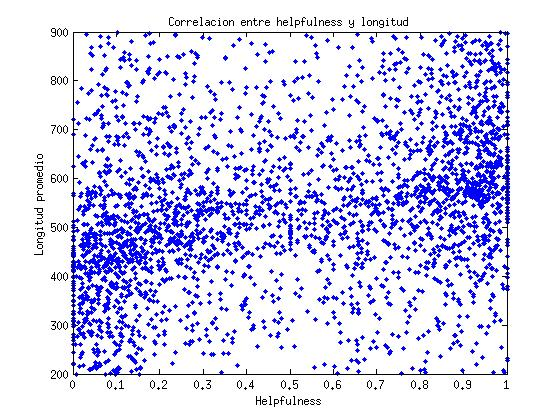
\includegraphics[scale=0.65]{corr.jpg}
\end{figure}

\section{Escalabilidad}

\subsection{Cloud Computing - Haas: Definicion}
La computacion en la nube son servidores - o granjas de servidores - repartidos por todo el mundo que alojan servicios de manera remota de forma tal que se puede acceder a un servicio contratado desde cualquier parte del mundo donde se disponga de una conexion a internet

La infraestructura como servicio (IaaS) o hardware as a service (HaaS) provee almacenamiento b\'asico y soluciones de c\'omputo como servicios contratables en la red.
Servidores, sistemas de almacenamiento, conexiones, routers, y otros sistemas se concentran a trav\'es de la tecnolog\'ia de virtualizaci\'on para manejar tipos espec\'ificos de cargas de trabajo. El ejemplo comercial mejor conocido es Amazon Web Services, cuyos servicios EC2 y S3 ofrecen c\'omputo y servicios de almacenamiento esenciales a clientes, de forma que puedan accederlos de forma sencilla y con alto grado de estabilidad. 

\subsection{Implementacion de nuestra solucion en la nube}
Existe un framework llamado Hadoop, que puede ayudarte a almacenar y procesar grandes volumenes de datos a cualquier escala, a traves de la distribucion de estos datos sobre una granja de servidores. El problema es que el lanzamiento, aprovisionamiento, manejo y configuracion de Hadoop puede ser complicado, costoso y puede tomar mucho tiempo valioso que puede aprovecharse analizando los datos. La forma mas comun de implementar esta idea, es comprar el servicio de \verb|hardware as a service (Haas)|, aprovisionar el hardware, instalar y finalmente lanzar el software sobre el hardware en la nube obtenido, todo esto sin poder siquiera haber procesado ningun dato aun.\\

\href{http://aws.amazon.com/es/elasticmapreduce/}{Amazon EMR} provee soluciones de facil uso, migracion y escalabilidad para el procesamiento de grandes cantidades de 
datos.
Amazon EMR, provee una forma simple, segura y rapida de solucionar este inconveniente: Aprovechando las plataformas \verb|Amazon EC2| y \verb|Amazon S3| se proveen soluciones de almacenamiento y procesamiento en la nube, brindando un entorno Hadoop que distribuye el procesamiento de los datos sobre multiples instancias de \verb|Amazon EC2|. Dado que \verb|Amazon EMR| permite trabajar con codigo \verb|map-reduce| personalizable, una vez obtenido el servicio, para comenzar, deben realizarse los siguientes pasos:
\begin{enumerate}
  \item Cargar los datos y aplicaciones de procesamiento dentro de \verb|Amazon S3|
  \item Distribuir los datos en la instancia de \verb|Amazon EC2|
  \item \verb|Amazon EMR| comienza a procesar los datos!
  \item Al finalizar el procesamiento, los resultados estaran disponibles en la instancia de \verb|Amazon S3|
\end{enumerate}

\subsection{Flexibilidad y costos}
\verb|Amazon EMR| monitorea el trabajo en todo momento, para desalojar los recursos en la nube al finalizar este, de esta forma, solo se paga por lo que se usa.
De manera facil, se puede incrementar o decrementar la cantidad de recursos para diferentes necesidades asociadas a volumenes de datos o necesidad de procesamiento mas rapido. El costo del servicio es flexible, puede pagarse por hora \verb|on-demand|, por capacidad fija reservada, entre otros. 

\subsection{Presupuesto y escalabilidad}
Dado que los volumenes de datos creceran a un ritmo lineal anual, y que \verb|map-reduce| tiene como premisa la escalabilidad lineal(por ejemplo: doble procesamiento - mitad de tiempo), Sean X el volumen de datos, Y la capacidad de procesamiento, Z el rendimiento obtenido en tiempo(mientras Z decrece, mayor rendimiento) y $k,t \in \mathbb{N}$, se tiene:
\newpage
\begin{center}
    Ecuacion de escalabilidad lineal para tama\~no fijo de datos: \\
    \textbf{$X$ datos en $t.Y$ hardware $\rightarrow$ $\frac{Z}{t}$ tiempo}
\end{center}
Asumiendo que el tiempo de procesamiento crece linealmente junto al tamaño de los datos, tenemos:\\
\begin{center}
    Ecuacion de escalabilidad lineal generalizada:\\
    \textbf{$k.X$ datos en $t.Y$ hardware $\rightarrow$ $\frac{k.Z}{t}$ tiempo}
\end{center}

Si queremos mantener el rendimiento Z constante, debemos incrementar linealmente en un factor k el hardware Y de forma anual de forma que la ecuacion se reestablezca:
\begin{center}
    Ecuacion de escalabilidad balanceada:\\
    \textbf{$k.X$ datos en $(k.t).Y$ hardware $\rightarrow$ $\frac{k.Z}{(k.t)}$ tiempo $\rightarrow$ $\frac{Z}{t}$ tiempo}
\end{center}

Respecto a la mejora obtenida respecto a utilizar una sola pc y utilizar los servicios en la nube es similar, dada la relacion de escalabilidad lineal, el rendimiento se mejorara linealmente a medida que incrementemos de forma lineal la cantidad de nodos en los clusteres de Amazon contratados.\\

En un caso hipotetico, dado que Amazon ofrece un clúster de Hadoop de 10 nodos por 0,15 USD la hora, habria que calcular los tiempos promedio de procesamiento requeridos, ajustar la cantidad de nodos segun el volumen, el tiempo necesario de procesamiento y hacer los calculos del gasto mensual, anual, etc del servicio requerido a Amazon. Siempre teniendo en cuenta que debe duplicarse anualmente la cantidad de nodos para mantener estable el rendimiento por lo mencionado en el parrafo anterior.


\end{document}